\documentclass[10pt, a4paper]{scrreprt}

	% TODO: export in Layout-File
	% parse into new layout!
	% create table of bibliography
	% Schriftgröße, Seitenränder, Abstand erhöhen --> erst zum Schluss ;-)

%% --------------------------- LAYOUT ------------------ %%
\usepackage[T1]{fontenc}
\usepackage[utf8]{inputenc}
\usepackage[ngerman]{babel}
\usepackage{amsmath}
\usepackage{amssymb}
\usepackage{selinput}
\usepackage{setspace}
\usepackage{geometry}
\usepackage{graphicx}
\usepackage{makeidx}

\SelectInputMappings{
 adieresis={ä},
 germandbls={ß},
}
\setlength{\topskip}{\ht\strutbox} % behebt Warnung von geometry
\geometry{paper=a4paper,left=30mm,right=20mm,top=20mm} 
\graphicspath{{pictures/}} % Specifies the directory where pictures are stored
\makeindex

%TODO: \onehalfspacing % Zeilenabstand erhöhen (1.5) 
% Seitenränder erhöhen!


%% ------------------------------------------------------ %%
%% ------------------------ BEGIN ---------------------- %%
%% -------------------------------------------------------%% 

\begin{document}


%% ---------------------------- TITLE ------------------------%%
\begin{titlepage}
\title{Implementierung einer Smartphone-Anwendung zum Austausch verschlüsselter Daten mit einer Cloud}
\maketitle
\end{titlepage}

% Text komplett in der Mitte von der Seite!
\vspace*{\fill}
\begin{center}
“If you think technology can solve your security problems, then you don’t understand the problems and you don’t understand the technology.”
\end{center}
\begin{flushright}
Bruce Schneier
\end{flushright}
\vspace*{\fill}


\tableofcontents

%% -------------------- EINLEITUNG ------------------ %%
\chapter{Einleitung}
% \setcounter{page}{1}
"Die Computer- und Internetnutzer in Deutschland setzen seit Bekanntwerden der geheimdienstlichen Abhöraktionen häufiger Verschlüsselungsverfahren ein." %[http://www.bitkom.org/files/documents/BITKOM-Presseinfo_Verschluesselung_18_12_2013_v2\%281\%29.pdf]
Aus der Pressemitteilung der BITKOM geht weiterhin hervor, dass von Juli 2013 auf November 2013 insgesamt 1,1 Millionen mehr Bundesbürger ihre persönlichen Dateien verschlüsseln. Besonders wichtig ist der Aspekt der Sicherheit, wenn es sich bei den Daten um relevante oder firmeninterne Informationen handelt, wie es z. B. am \index{Deutschen Elektronen Synchrotron (DESY)} in Hamburg der Fall ist. Auch der Austausch von Daten von mobilen Endgeräten wie \index{Smartphones} oder Tables spielen eine immer größere Rolle wie die Entwicklung der letzten Jahre zeigt (siehe Grafik). \\ 
\begin{center}
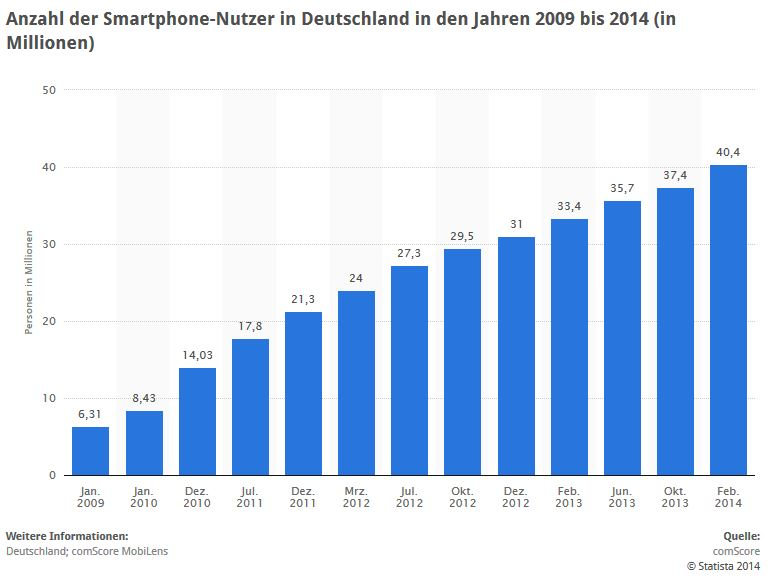
\includegraphics[scale=0.6]{smartphoneUser_Germany.JPG} %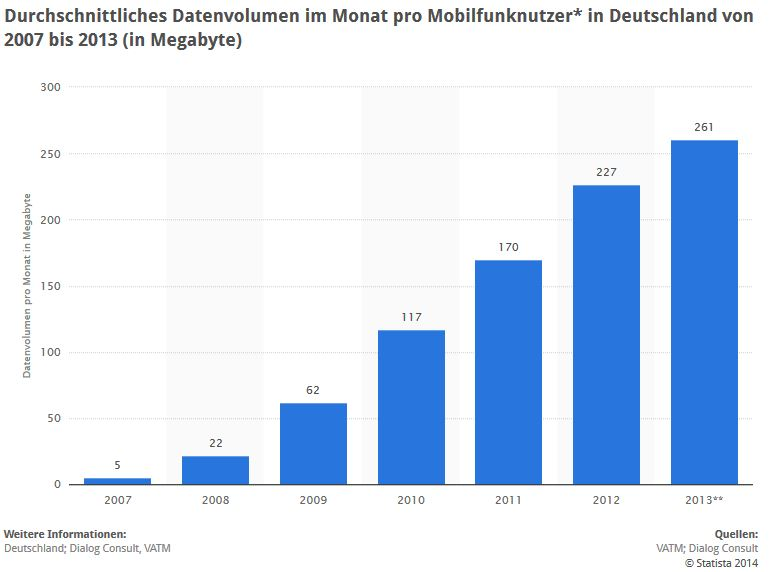
\includegraphics[scale=0.40]{datatraffic_germany.JPG} % zweite Grafik evtl. an anderer Stelle passender?
\end{center}
Herkömmliche Verfahren zum Austausch von Daten reichen oftmals nicht mehr aus, wenn man den Aspekt der Sicherheit näher beleuchtet. % TODO: prüfen? kann man das so stehen lassen?!?


\section{Motivation}
Am Deutschen Elektronen Synchrotron, im folgenden DESY, werden bisher wichtige und sensible Dokumente über ein Programm Namens Dropbox gesichert und verwaltet. Dropbox bietet eine plattformunabhänginge Möglichkeit Dokumente Online abzuspeichern und von einem anderen Standort über ein internetfähiges Gerät wieder zu öffnen [https://www.dropbox.com/]. Auch wenn Dropbox nach eigenen Angaben den Advanced Encryption Standard (AES)  verwendet, bevor die Daten gespeichert werden, liegen die dafür notwendigen Schlüssel in Händen der Betreiber selbst, die somit vollen Klartextzugriff auf die Nutzerdateien haben. Dropbox begründet diesen Zugriff wie folgt:  "Wie die meisten Online-Dienste verfügt auch Dropbox über einen kleinen Mitarbeiterstamm, dem aus in unserer Datenschutzrichtlinie dargelegten Gründen Zugriffsrechte auf Nutzerdaten gewährt werden muss [...]". \\ % TODO [https://www.dropbox.com/help/27/de aufgerufen 01.07.2014]
Da das DESY über eine eigene Cloud-Infrastruktur verfügt, sollen in Zukunft alle wichtigen Daten nicht nur in dieser Cloud gespeichert werden, sondern auch zusätzlich durch eine Verschlüsselung gesichert werden. Die Cloud am DESY stellt im Hintergrund ein Rechnernetz zum Abspeichern von Daten zur Verfügung. Durch das Programm dCache, welches das Rechnernetz im Hintergrund steuert und verwaltet, ist es dem Anwender möglich Daten in das System zu speichern, ohne dessen Struktur zu kennen. dCache sorgt dafür dass die Daten, je nach Bedarf, mehrfach abgelegt werden und bei einem Zugriff schnell zur Verfügung stehen. Die Dateien selbst werden im Hintergrund auf verschiedene Datenträger, wie z. B. SSD-Festplatten, Magnetbänder, Tapes o. ä., abgelegt. Das System sorgt dafür, dass bei reger Anfrage die Daten, sofern möglich, auf ein schnelleres Medium repliziert werden. Die genaue Struktur und Vorgehensweise des Programmes ist jedoch nicht Teil dieser Arbeit, da das hier zu entwickelnde Programm nur die Schnittstelle des dCache-Servers verwendet.


\section{Zielsetzung}
Ziel dieser Arbeit ist es aus diesem Grund einen Prototyp zu entwickeln, der einerseits mit dem Cloud-System des DESY Kommunizieren kann um dort Dateien hoch- und herunter zu laden, andererseits diese Daten auch in angemessener Form (siehe Kapitel Validierung) zu Verschlüsseln. \\
In der ersten Version dieser Arbeit wird ein Programm entwickelt, welches auf Android-Betriebssystemen zum Einsatz kommen kann. Darüber hinaus ist es wichtig, dass die entsprechenden Schlüssel zum entschlüsseln der Daten nicht zusammen mit den Daten abgelegt werden, sondern ausschließlich den Parteien des Datenaustauschs bekannt sein soll. Dies bedeutet, das selbst die Betreiber am DESY nicht die Möglichkeit haben die abgelegten Daten zu entschlüsseln. \\
Zum Ver- und Entschüsseln der Daten sollen Verfahren verwendet werden, die in der heutigen Zeit als sicher angesehen werden und Smartphones im Bezug auf Performance und Akkuverbrauch nicht zu stark belasten. Um diese Faktoren zu Validieren wird eine Testanwendung geschrieben, die mit bestimmten Faktoren die verschiedenen Verfahren untereinander überprüfen (siehe Kapitel Validierung).

	% TODO: Prüfen, ob dieser Part wirklich hier rein muss? Andere Software vergleichen?
\section{Verwandte Arbeiten}
	% TODO: Recherche?!? --> wird nicht benötigt, da es sich bei der Arbeit hautpsächlich um die Entwicklung des Programmes handelt. Kryptographische Verfahren wurdne zu genüge behandelt.
\section{Verwandte Programme}
	% TODO: Unterscheidung in Arbeiten & Programme notwendig?
	% vgl. Dropbox
	% vgl. ownCloud <<- speziell: soll in Zukunft am DESY verwendet werden --> kompatiblität beachten?!? 
	% vgl. boxcryptor
	% vgl. cloudfogger


\section{Diese Arbeit}
\subsection{Inhaltlicher Aufbau}

% \chapter{Anforderungen} ?


%% ---------------------- GRUNDLAGEN ----------------- %%
\chapter{Grundlagen Android}
Android ist ein Betriebssystem für Smartphones und Tablets, welches von der open handset alliance entwickelt wird. Das Konsortium besteht aktuell aus 84 Unternehmen, die an der Entwicklung des Betriebssystems arbeiten. %http://www.openhandsetalliance.com/index.html]
In diesem Kapitel wird kurz darauf eingegangen, welche Kryptografischen Aspekte Android in den verschiedenen Versionen zur Verfügung stellt um diese im darauffolgenden Kapitel genauer zu Untersuchen. Aufgrund der Tatsache, dass die Android Version Gingerbread (2.3.3) im Juni 2014 noch einen Marktanteil von knapp 15\% hält, ist dies auch die niedrigste vom Programm unterstützte Version. \\
\begin{center}
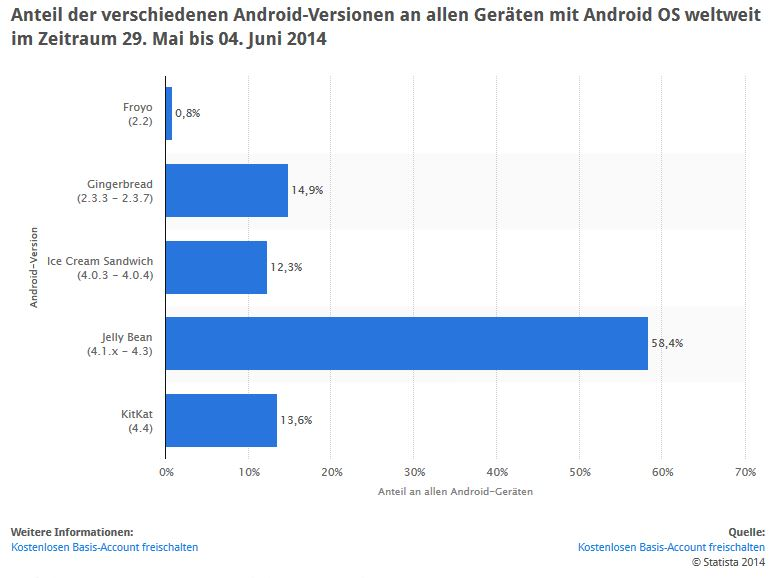
\includegraphics[scale=0.6]{android_version_marktanteil.JPG} %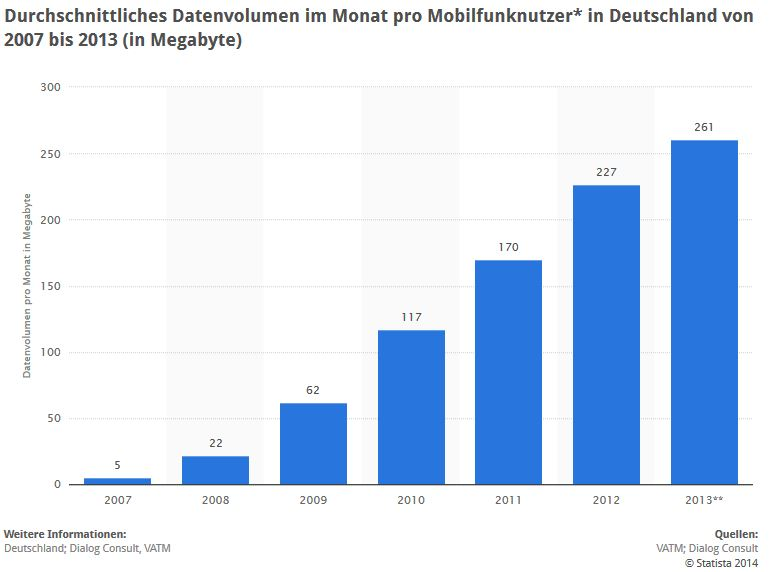
\includegraphics[scale=0.40]{datatraffic_germany.JPG} % zweite Grafik evtl. an anderer Stelle passender?
\end{center}
Bei der Analyse wird darauf geachtet, dass alle Funktionalitäten die im Programm entwickelt werden, von dieser Version unterstützt werden. Die, während des Schreibens dieser Arbeit, aktuellste Version der Android API ist KitKat (4.4), bei der darauf geachtet wird, dass die eingesetzten Funktionen auch in dieser Version noch zur Verfügung stehen und nicht mit \textit{deprecated (veraltet)} markiert sind.


\section{Zusammenhang Kryptographie}
Beim Thema Sicherheit im Zusammenhang mit Android ist erstmals der Begriff der Sandbox zu nennen. Eine Anwendung wird abgekapselt in einer eigenen Umgebung mit eigenem Prozess, eigenem Betriebssystem-User, eigener Dalvik-VM, eigenem Heap und eigenem Dateisystem ausgeführt. Dieses abgekapselte Konstrukt wird Sandbox bezeichnet. Dadurch ist es dem Betriebssystem möglich unerlaubten Zugriff auf Ressourcen oder andere Programme zu beschränken, hierbei wird das Berechtigung- und Prozess-Management-System von Linux verwendet. %Becker, Arno Android 4.4 - Seite 33]
Um dennoch verschiedene Zugriffe zu erlauben muss in der sogenannten Manifest-Datei der Anwendung die Berechtigung festgelegt und vom Benutzer bei der Erstinstallation bestätigt werden.
Auch wenn dieses Konzept Daten zur Laufzeit innerhalb einer Anwendung schützt, ist es möglich Dateien auch auf einer SD-Karte zu speichern, in das Internet zu verschicken oder über andere Wege auszutauschen. Diese Daten sind dann außerhalb der Anwendung und gegen externe Zugriffe nicht mehr geschützt.
Dennoch gibt es die Möglichkeit in Android diese Daten zusätzlich mit einer Verschlüsselung zu versehen - hierfür stellt Java, seit der Version 1.4, die \textit{Java Cryptography Extension (JCE)} innerhalb von Android zur Verfügung. Innerhalb der Erweiterung (engl. extension) sind verschiedene Provider eingebunden, die dem Programmierer die Möglichkeit geben Kryptografische Verfahren aufzurufen, ohne die genaue Implementierung kennen zu müssen. In Java-Anwendungen gibt es diverse Implementierungen von Sun, die jedoch aus Datenschutzrechtlichen Gründen nicht in der Android Java-API vorhanden sind. der Provider Bouncy-Castle stellt eine Alternative zur Implementierung von Sun darf und wird in Android zur Verfügung gestellt. Innerhalb von Android wurde das Paket so geändert, dass es den Richtlinien der JCE entspricht. 
Bouncy-Castle ist einer der von Android zur Verfügung gestellten Provider - jedoch gibt es noch weitere Provider, die selbige oder andere Implementierungen zur Verfügung stellen. Mit folgendem Codeabschnitt ist es möglich die einzelnen Provider mit den unterstützten Verfahren auszulesen und untereinander zu vergleichen. Dieser Code wurde auf verschiedenen Versionen ausgeführt, um die Unterschiede der einzelnen Versionen hervorzuheben. \\
\begin{center}
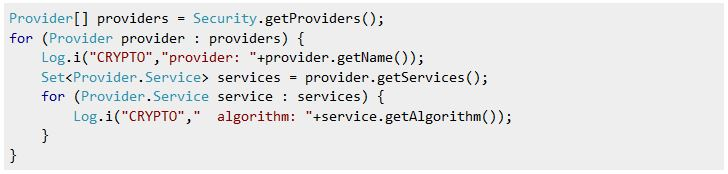
\includegraphics[scale=0.8]{read_cryptoprovider.JPG} %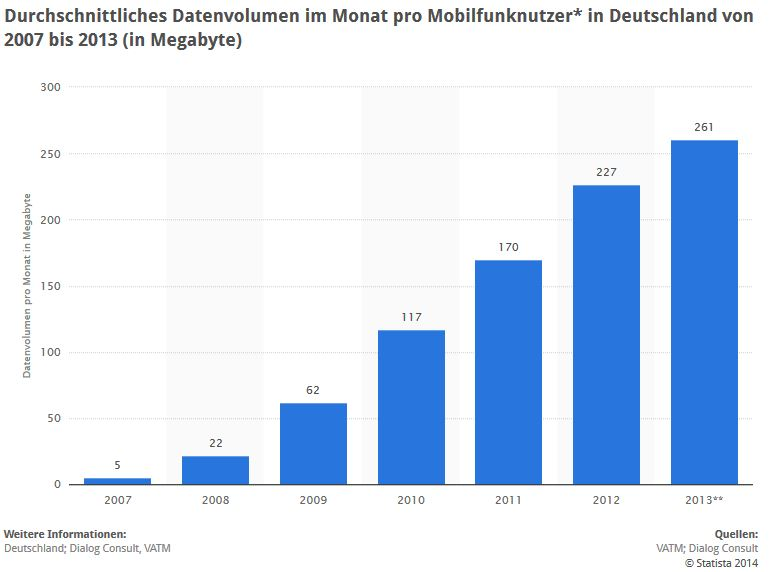
\includegraphics[scale=0.40]{datatraffic_germany.JPG} % zweite Grafik evtl. an anderer Stelle passender?
\end{center}
Im Vergleich stehen folgende Android-Versionen:
\shorthandoff{"}
\begin{itemize}
\item 2.3.3 (Gingerbread) : die niedrigste vom Programm unterstützte Version
\item 4.1.1 (Jelly Bean) : die Version des Entwickler-Gerätes
\item 4.4.4 (KitKat) : aktuellste auf dem Markt verfügbare Android-Version
\item "L" : zukünftige Version, welche bereits zu Testzwecken als Entwickler-Version freigeschaltet ist. Der Codename "L" zeigt auf, dass es sich in der Folge der Süßigkeiten (Gingerbread, HoneyComb, Ice Cream Sandwich, Jelly Bean, KitKat) vermutlich alphabetisch fortsetzen wird - die Versionsnummer ist bis dato nicht bekannt.
\end{itemize}
Im Vergleich der Ausgabe eines Gerätes mit Android 2.3.3 und eines mit 4.1.1 bzw. 4.4.4 und "L" liegt der Hauptunterschied in der Unterstützung von Elliptischen Kurven für das Diffie-Hellmann-Verfahren (ECDH) und den Digital-Signature-Algorithm (ECDSA), welche in der Version 2.3.3 nicht unterstützt werden. Des Weiteren ist ab der Version 4.4.x der Provider OpenSSL und deren Algorithmen spezifischer dargestellt.
Folgende Verschlüsselungsverfahren werden sowohl von der Version 2.3.3 als auch von der Version 4.1.1 , 4.4.4 und L unterstützt und werden im nachfolgenden Kapitel näher erläutert: \\ \\
\begin{tabular}{|l|l|} \hline\hline
\textbf{Verschluesselung} & \textbf{Hash-Funktion} \\ \hline &  \\
AES & MD5 \\
ARC4 & SHA1 \\
Blowfish & SHA256 \\
DES & SHA384 \\
3DES & SHA512 \\
PBE & \\
RSA & \\
\hline\hline
\end{tabular} \\
\\Des Weiteren wird das Key-Wrap-Verfahren (AES und 3DES), der Authentifizierungsalgorithmus HMAC und der Standard X509 beschrieben. Die Vollständige Liste aller Unterstützen Algorithmen mit dessen Providern befindet sich im Anhang. Welcher Provider für welchen Algorithmus besser geeignet ist, kann man nicht pauschalisieren und auch nicht auf einen spezifischen Anwendungsfall verallgemeinern. Im Kapitel Validierung werden Geschwindigkeitsaspekte beider großen Provider (OpenSSL und Bouncy-Castle), sofern möglich, gegenübergestellt um für jeden Algorithmus den geeigneten Provider zu wählen. Falls es innerhalb eines Providers zu größeren Sicherheitslücken von einem verwendeten Algorithmus kommt, ist es durch das JCE möglich diesen ohne weitere Code-Änderungen zu wechseln. 


\chapter{Grundlagen Kryptologie}
Das Wort Kryptologie stammt aus dem Griechischen \textit{kryptós} für verstecken und \textit{lógos} für die Lehre.% [Duden http://www.duden.de/rechtschreibung/krypto_, http://www.duden.de/rechtschreibung/_logie] 
Dieser Zweig umfasst die Kryptographie - die Wissenschaft die sich mit der Absicherung von Daten beschäftigt, die Kryptoanalyse - welche für das Aufbrechen von Geheimnachrichten zuständig ist sowie der Mathematik.
Im Bereich der Kryptologie ist es das Ziel eine Nachricht, welche aus lesbaren Zeichen (Klartext) besteht unverständlich zu machen (Verschlüsseln) und daraus einen Geheimtext (Chiffretext) zu erzeugen. Dieses Verfahren wird mit mathematischen Funktionen und einem Schlüssel (Key) durchgeführt. Die Umkehrung von Chiffretext in Klartext (Entschlüsselung) wird ebenfalls durch eine mathematische Funktion und einen Schlüssel durchgeführt. Ziel dieser Ver- und Entschlüsselung ist es Nachrichten zwischen einem Sender und Empfänger so auszutauschen, dass ein Angreifer diese nicht mitlesen, oder im verschärftem Sinne nicht verändern kann. Hierbei besteht eine Nachricht in der Informatik immer aus binären Daten und kann eine Textdatei, ein Bild, ein Video oder vieles mehr darstellen. Ver- und Entschlüsselung sind mathematische Funktionen, die auf den Klartext, bzw. auf den Chiffretext angewendet werden. 


\subsubsection{Terminologie}
Um die Lesbarkeit zu erhöhen wird Klartext im folgenden mit M (engl. Message), Chiffretext mit C (engl. Chiffre), die Verschlüsselungsfunktion mit E (engl. Encoding), die Entschlüsselungsfunktion mit D (engl. Decoding) und dem Schlüssel K (engl. Key) beschrieben.
Zum Verschlüsseln kommt also folgende Funktion zum Einsatz: \\ \\
E$_{K}$(M) = C\\ \\ 
Um den Chiffretext wieder zu Entschlüsseln wird die umgekehrte Richtung angewandt:\\ \\
D$_{K}$(C) = M\\ \\
Zusammengefasst muss also gelten: das Verschlüsseln einer Nachricht und das darauffolgende Entschlüsseln des erzeugten Chiffretextes, mit der dazugehörigen Funktion und korrektem Schlüssel, muss wieder den Klartext ergeben. Mathematisch beschrieben ist das wie folgt:\\ \\
D$_{K}$(E$_{K}$(M)) = M\\ \\
Um einen sicheren Kanal zwischen Sender und Empfänger zu gewährleistet, reicht es nicht allein die Nachricht zu verschlüsseln. Authentifizierung, Integrität und Verbindlichkeit müssen darüber hinaus gewährleistet sein um sicher zu Kommunizieren. \\ \\
\textbf{Authentifizierung} beschreibt hierbei das Verfahren indem sich die Identität einer Person beweisen lässt. Im Umkehrschluss bedeutet das, dass sich ein Angreifer nicht als eine andere Person ausgeben kann. Aus der Authentifizierung folgt dann die \textbf{Autorisierung}, also das Prüfen, ob der Benutzer die Rechte hat, die er fordert.\\ \\
\textbf{Integrität} bedeutet, dass sichergestellt werden kann, dass eine Nachricht bei der Übermittlung zwischen Sender und Empfänger nicht durch einen Angreifer verändert wurden ist. \\ \\
\textbf{Verbindlichkeit} beschreibt  dass der Sender nicht leugnen kann, dass eine Nachricht gesendet wurde. \\ \\


\subsubsection{Kerhoff's Maxime}
Ein Aspekt in der Kryptographie sind die Kerkhoffs' Maxime, die folgendes Aussagen: "the security of the encryption scheme must depend only on the secrecy of the Key K$_{e}$, and not on the secrecy of the algorithms." [Schneier, 1997] Übersetzt bedeutet es, dass die Sicherheit eines Kryptographischen Verfahrens  auf der Geheimhaltung des Schlüssels beruhen muss und nicht auf derer des Verschlüsselungsalgorithmus.


\subsubsection{Verfahren}
Prinzipiell unterteilt man Kryptographie in zwei Verschiedene Verfahren. Die symmetrischen Verfahren und die asymmetrischen, auch public key infrastructure genannt. Generell lässt sich über das "bessere Verfahren" keine Aussage treffen, da es für beide Verfahren Vor- und Nachteile gibt. Bruce Schneier fasste es wie folgt zusammen: \\
"Symmetrische Kryptographie eignet sich am besten zur Verschlüsselung von Daten. Sie ist um Größenordnungen schneller und nicht anfällig für chosen-ciphertext-Angriffe. Public-Key-Kryptographie schafft Dinge, die außerhalb des Einsatzbereichs symmetrischer Kryptographie liegen und eignen sich am besten für die Schlüsselverwaltung und eine Vielzahl der Protokolle [...]."\\ %[Schneier, 1996 übersetzt, Seite 254f]
Der im Zitat verwendete Ausdruck, chosen-ciphertext-Angriff beschreibt einen Angriff auf ein Kryptosystem, bei dem der Kryptoanalytiker verschiedene Chiffretexte zur Entschlüsselung auswählen kann und entsprechend Zugriff auf den dazugehörigen Klartext besitzt. Die Aufgabe bei dieser Art des Angriffes besteht darin, den entsprechenden Schlüssel herauszufinden. %[Schneier 1997, Seite 7]
Neben der chosen-ciphertext-Angriffe gibt es weitere Angriffsszenarien auf Kryptosysteme, wie z. B. ciphertext-only, known-plaintext, chosen-plaintext, chosen-key und weitere. Da es sich bei dieser Arbeit nicht um eine Kryptoanalyse eines Systems handelt, werden diese Szenarien nicht näher erläutert. Es wird davon ausgegangen, dass wenn eines dieser Szenarien zum knacken des Systems führt, dieses kryptographische Verfahren bereits heute als unsicher angesehen wird.


\section{Symmetrische Verfahren}
	% DES --> AES ist der Nachfolgder, deswegen keine weitere Behandlung.
Bei symmetrischen Verschlüsselungsverfahren existiert ein Schlüssel, der jeweils für Ver- und Entschlüsselung verwendet wird. Dieser Schlüssel muss bereits beiden Parteien bekannt sein, bevor ein verschlüsselter Kanal aufgebaut werden kann. Eines der Probleme bei symmetrischen Verfahren ist der Austausch des Schlüssels, den man von Sender zu Empfänger, bereits vor der sicheren Kommunikation, übertragen muss (siehe Kapitel Schlüsselvereinbarung). Symmetrische Verfahren unterteilt man in zwei Grundtypen, die Block- und Stromchiffrierung. Bei der Blockchiffrierung wird der Klartext in Blöcke, mit fester Größe, aufgeteilt und innerhalb des Blockes werden die mathematischen Funktionen angewandt. Bei der Stromchiffrierung werden die Daten nicht in Blöcken zusammengefasst, sondern jedes einzelne Klartextbit wird in ein Chiffrebit überführt. [Schneier 1996, Seite 223] 


\subsection{DES, 3DES}
"Its restricted key size of 56 bits and small block size of 64 bits make it unsuitable for today`s fast computers and large amounts of data. It survives in the form of 3DES, which is a block cipher built from three DES encryptions in sequence. This solves the most immediate problem of the small key size, but there is no known fix for the small block size. [...] we do not recommend using either DES oder 3DES in new designs." [Ferguson 2003, Seite 51]
Niels Ferguson weißt darauf hin, dass DES aufgrund seiner Schlüsselänge von 56 bits und der Blockgröße von 64 bits ungeeignet für heutige Systeme ist. Weiterhin beschreibt er, dass auch durch 3DES das Problem der geringen Blockgröße nicht behoben wird und er schlussfolgert dass man in heutigen neuen Systemen beide Verfahren nicht verwenden sollte. \\
Da das System als unsicher angesehen ist, wird auf eine nähere Untersuchung und Erläuterung der mathematischen Funktionen verzichtet. DES und 3DES wird in der zu entwickelnden Anwendung nicht implementiert.

\subsection{AES}

\subsection{ARC4}
\subsection{PBE}


\section{Asymetrische Verfahren}
\subsection{RSA}

\section{Hash-Funktionen}
\section{Digitale Signature}
\subsection{Public Key Infrastruktur}
\section{Schlüsselvereinbarung}
\subsection{Diffie Hellmann}
\subsection{ElGamal}
\section{Schlüsselgenerierung}
\section{Authentifizierung}
\subsection{Zwei-Faktor-Authentifizierung}
	% TODO: Erklärung: http://de.wikipedia.org/wiki/Zwei-Faktor-Authentifizierung (need Quelle)


%% ------------------------ VALIDIERUNG --------------------- %%
\chapter{Validierung}
	% TODO: Erläuterung des Testgerätes & der Punkte auf die getestet werden soll!
	% aufzeigen der Notwendigkeit dieser Validierung
\section{Verschlüsselungsverfahren}
\section{Hashfunktionen}

%% ------------------------ IMPLEMENTIERUNG ---------------- %%
\chapter{Implementierung}
\section{Entwurf}

%% ----------------------------- TEST -------------------------- %%
\chapter{Test}
\section{Validierung}
\section{Testverfahren}

%% -------------------------- ZUSAMMENFASSUNG -------------- %%
\chapter{Zusammenfassung und Ausblick}
\section{Zusammenfassung}
\section{Ausblick}

%--------------------------------------------------------------------
% -----------------------ENDE ------------------------------------
%------------------------------------------------------------------


%% --------------------------- BIBLIO --------------------------------%%
%\label{Bibliography}

%\lhead{\emph{Bibliography}} % Change the page header to say "Bibliography"

%\bibliographystyle{unsrtnat} % Use the "unsrtnat" BibTeX style for formatting the Bibliography

%\bibliography{Bibliography} % The references (bibliography) information are stored in the file named "Bibliography.bib"

\printindex

%Glossar
%Literatur
%Diagramme
%Tabellen
%eigenständigkeitsverklärung

%% ---------------------------------- ANHANG --------------------------- %%
	%TODO: Algorithmen 411 und 322.

\end{document}